\xchapter{Sustentabilidade do ecossistema de software acadêmico de análise estática}
{Este capítulo apresenta a avaliação do ecossistema de software acadêmico de
análise estática quanto à sua sustentabilidade técnica, ou seja, a capacidade
de perdurar, de continuar disponível no futuro, e a sua manutenabilidade.}

\section{Avaliação da sustentabilidade técnica}

\label{sustentabilidade-tecnica}

% Introduction
% Background
% Experimental Setup (hipoteses / design)
% Results (data analysis)
% Discussion
% Threats to validity
% Conclusions

%apesar disso, antes mesmo de resolver tais questões é
%fundamental compreender os impactos que eles causam na comunidade de pesquisa.

Este estudo tem como objetivo medir e avaliar a sustentabilidade técnica dos
softwares acadêmicos de análise estática publicados na literatura acadêmica.

\subsection{Planejamento do estudo}

...

\subsection{Questões de pesquisa}

Neste estudo as seguintes questões de pesquisa serão investigadas:

\newcommand{\QuestaoUm}{Na literatura científica publicada, como as taxas de
softwares publicados, no domínio de aplicação de análise estática, mudam ao
longo do tempo?}

\newcommand{\QuestaoDois}{Os softwares acadêmicos de análise estática, publicados
na literatura científica, estão disponíveis para obtenção hoje?}

\newcommand{\QuestaoTres}{Na literatura científica publicada, como as taxas de
softwares disponíveis, no domínio de aplicação de análise estática, mudam ao
longo do tempo?}

\newcommand{\QuestaoQuatro}{Podemos adaptar de forma incremental os softwares
acadêmicos de análise estática para aproveitar oportunidades emergentes, sem
perda de reprodutibilidade?}

\begin{description}
  \item [Q1:] \QuestaoUm
  \item [Q2:] \QuestaoDois
  \item [Q3:] \QuestaoTres
  \item [Q4:] \QuestaoQuatro
\end{description}

\subsection{Seleção de softwares acadêmicos}

Os softwares foram selecionados através de uma {\it revisão estruturada}, um processo disciplinado
para busca e seleção de softwares de um domínio específico publicados em
artigos acadêmicos, usando critérios bem definidos, de forma que seja
possível a reprodução do estudo por parte de pesquisadores interessados.

%A revisão estruturada difere da revisão e do mapeamento sistemático
%\cite{Kitchenham2007} por ser um processo mais simples e menos rígido, onde o
%resultado final é um conjunto de softwares, enquanto no mapeamento ou na
%revisão sistemática há um esforço em caracterizar os artigos analisados o mesmo
%não ocorre na revisão estruturada, onde o esforço reside em caracterizar os
%softwares acadêmicos.

Seguem detalhes de cada atividade:

\begin{description}

  \item[(1) Busca] ...

  \item[(2) Filtro]

  \item[(3) Seleção]

\end{description}

Ao final da revisão poderemos responder à questão de pesquisa {\bf Q1}
(\QuestaoUm) usando os dados dos softwares acadêmicos selecionados.

\subsection{Quantificação da disponibilidade dos softwares acadêmicos}

Os softwares acadêmicos selecionados na revisão estruturada foram avaliados em
relação à sua disponibilidade, apenas os softwares com indicação de fonte para
obtenção foram incluídos, dois aspectos foram analisados, um relacionado à como
o artigo cita o software e outro relacionado a como o software está disponível,
código fonte, binários e licença utilizada.

O primeiro aspecto tem o objetivo de identificar se o software está disponível
de fato, se o endereço está acessível publicamente e se é possível obter uma
cópia do software, cada software acadêmico será caracterizado entre uma das
seguintes opções:

\begin{itemize}
  \item Fonte para obtenção do software indisponível -
    {\it O artigo indica fonte mas encontra-se inacessível, fora do ar ou com erros}
  \item Software disponivel, binários ou código fonte -
    {\it A fonte indicada está disponível e acessível publicamente}
\end{itemize}

O endereço indicado no artigo será acessado a fim de identificar se está
funcional e se é possível obter uma cópia do software, essa avaliação nos dirá
o quanto permanecem disponíveis os softwares publicados na literatura
acadêmica, lembrando que pequenos scripts ou protótipos sem indicação de
endereço para obtenção não foram considerados neste estudo, a revisão
estruturada, responsável pelo conjunto de softwares selecionados, preocupa-se
apenas em encontrar softwares acadêmicos citados pelo autor como uma das
contribuições do seu estudo, e que tenha sido indicado endereço para obtenção do
mesmo.

Isto nos permitirá responder as questões de pesquisa {\bf Q2} (\QuestaoDois)
e {\bf Q3} (\QuestaoTres).

%Mesmo que o autor tenha disponibilizado fontes para obtenção dos artefatos produzidos,
%o fato de não informarem a fonte inviabiliza, ou ao menos dificulta, bastante
%pesquisadores interessados em repetir ou reproduzir os resultados de tais estudos.

O segundo aspecto investigado diz respeito à como os softwares estão disponíveis,
serão caracterizados como:

\begin{itemize}
  \item Código fonte disponível
  \item Apenas binários disponível
\end{itemize}

%Esse segundo aspecto toma como base o trabalho de \citeonline{Novak2010} em que
%propõe uma taxonomia e um conjunto de dimensões para caracterização de
%ferramentas de análise estática, uma das dimensões para caracterização
%é esta relacionado à como o software é disponibilizado.
%
%Os softwares caracterizados como {\it ``código fonte disponível''} incluirão
%qualquer softwares mesmo sem licença definida,
%
%segundo as definições de software {\it
%livre} e {\it open} da Free Software
%Foundation\footnote{\url{https://www.gnu.org/philosophy/free-sw.html}} e Open
%Source Initiative\footnote{\url{https://opensource.org/osd}}, respectivamente,

Não estamos avaliando se os softwares são livres ou de código aberto, portanto
os softwares com código fonte incluirão tanto softwares com licença definida
quanto softwares sem licença, a disponibilidade e o acesso ao código fonte
possibilita aos interessados estudar e absorver o conhecimento empregado nestes
softwares, um conhecimento muitas vezes altamente especializado e útil para a
comunidade científica.

A avaliação sobre a disponibilidade de código fonte nos permitirá responder a questão de pesquisa
{\bf Q4} (\QuestaoQuatro).

A fonte para coleta dessas informações serão os artigos relacionados aos
softwares, código fonte, documentos e site do projeto, quando disponíveis.

\subsection{Quantificação da disponibilidade dos softwares acadêmicos}

\section{Resultados}

Todas as trilhas de ambas as conferências
foram incluídas, encontramos nesta atividade 1873 artigos no total, 1527 artigos
do ASE e 346 artigos do SCAM, com uma média geral de 75 artigos publicados por ano. A
Figura \ref{artigos-por-ano} apresenta a distribuição por edição de cada
evento.

(1) Busca -- Todas as trilhas de ambas as conferências foram incluídas,
encontramos nesta atividade 1873 artigos no total, 1527 artigos do ASE e 346
artigos do SCAM, com uma média geral de 75 artigos publicados por ano. A Figura
\ref{artigos-por-ano} apresenta a distribuição por edição de cada evento.

\begin{figure}[h]
  \center
  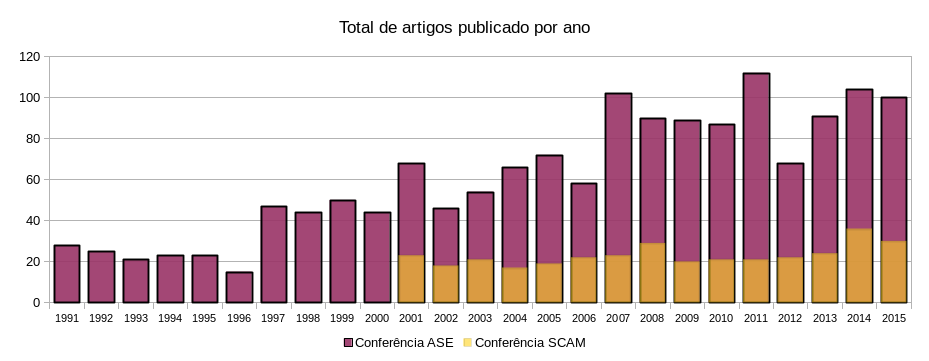
\includegraphics[scale=0.65]{imagens/artigos-por-ano.png}
  \caption{Gráfico em barras com o total de artigos publicado por ano}
  \label{artigos-por-ano}
\end{figure}

Entre os anos de 1991 e 1996 a conferencia ASE chamava-se KBSE - {\it
Knowledge-Based Software Engineering Conference} e só a partir de 1997 passou a
chamar-se ASE - {\it Automated Software Conference}. A edição com o maior
número de publicações foi 2011 com 112 artigos publicados, seguido de 2014 com
104, e 2007 com 102, a edição com o menor número foi 1996 com apenas 15 artigos
publicados.

A conferência SCAM teve sua primeira edição apenas em 2001, 10 anos após a
primeira edição do ASE, e possui uma média de 23 artigos publicados por edição.
Se compararmos os mesmos períodos de ambas as conferências, 2001 à 2015,
percebemos que a conferência ASE publica quase 4 vezes mais do que a
conferência SCAM. Neste período a conferência ASE teve uma média de 80 artigos
publicados por ano, se for levado em conta todas as edições, apenas da
conferência ASE, a média cai para 61 artigos por ano.

(2) Filtro -- reduziu em 77\%
o número total de artigos, resultando em 441 artigos
para serem analisados na próxima etapa da revisão estruturada.  Durante a execução desta
atividade foi necessário analisar dois artigos manualmente, {\it Adaptable
concern-based framework specialization in UML} e {\it Property-oriented test
generation from UML Statecharts}. O conteúdo destes dois artigos não é possível
de ser analisados pelo script de filtro uma vez que é formado por imagens
digitalizadas, ambos artigos publicados no ASE edição 2004. Nenhum dos dois
artigos continham os termos pesquisados e ficaram fora do conjunto selecionado
nesta atividade.

A terceira e última atividade da revisão estruturada -- (3) Seleção --
realizada em cima dos 441 artigos selecionou 107 artigos com publicação de
software científico do domínio de aplicação de análise estática, alguns destes
artigos fazem referência à um mesmo software, é o caso do {\it BEST: A symbolic
testing tool for predicting multi-threaded program failures} e do {\it Scalable
and precise symbolic analysis for atomicity violations}, ambos publicados no
ASE 2011 fazem referência ao software BEST. Situação similar ocorreu com o {\it Augmenting
Counterexample-Guided Abstraction Refinement with Proof Templates} e o {\it
PtYasm: Software Model Checking with Proof Templates} publicados no ASE 2008,
fazem referência ao software PtYasm. Por conta disso, entre os 107 artigos, temos
105 softwares distintos, uma lista com todos os softwares e uma breve descrição
de cada um é apresentado no Apêndice \ref{resumo-softwares},
detalhes sobre o número de artigos e softwares encontrados em cada conferência
pode ser consultados nos Apêndices \ref{artigos-do-scam} e \ref{artigos-do-ase} 

Ainda durante esta última atividade da revisão cada um dos 107 artigos foram
analisados em busca de informações sobre onde encontrar o software indicado,
esta análise resultou em 60 softwares com indicação de fonte para obtenção do
software, apenas os artigos que indicam endereço de página web para download do
software foram selecionados, ou seja, uma grande parte dos artigos que produzem
softwares acadêmicos nem ao menos citam o software no paper, ou quando citam,
não informam site ou endereço do projeto para download
\cite{allen2017engineering}, seja código fonte ou apenas binários. A Figura
\ref{softwares-por-ano} apresenta os 60 softwares distribuídos ao longo dos
anos num gráfico em linha.

\begin{figure}[h]
  \center
  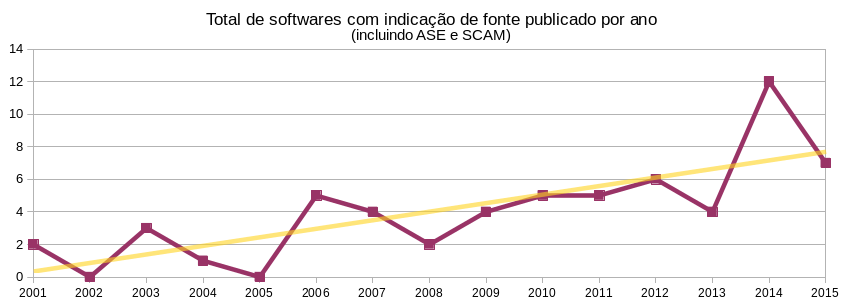
\includegraphics[scale=0.65]{imagens/softwares-por-ano.png}
  \caption{Gráfico em linha com o número de softwares por ano selecionados na revisão estruturada}
  \label{softwares-por-ano}
\end{figure}

É possível perceber um certo crescimento no número de softwares publicados com
o passar dos anos, ao menos em softwares do domínio de análise estática, de
forma que podemos confirmar que considerando as conferências ASE e SCAM, há um
crescimento na publicação de softwares acadêmicos ao longo do tempo, nos dando
oportunidade de responder parte da questão de pesquisa {\bf Q1} (\QuestaoUm).

Apesar da busca na atividade -- (2) Filtro -- utilizar termos com o objetivo de
encontrar apenas softwares disponíveis com informação de onde encontrar o
software, ainda assim, encontramos 45 artigos com publicação de software sem
indicação de fonte para obtenção.

Entre os 1873 artigos, encontramos 107 artigos referenciando 105 softwares de
análise estática, apenas 60 destes indicam fonte onde o software pode ser
encontrado, apenas 37 estão disponíveis, os 23 restantes indicam fonte não mais
acessíveis, endereço não encontrado, indisponível, ou com informações não
relacionadas ao software. O Apêndice \ref{resumo-softwares-disponiveis} traz
uma tabela com os nomes e endereços web onde os softwares estão disponíveis.

Esta informação nos permite responder a questão de pesquisa {\bf Q2}
(\QuestaoDois), levando em conta a sustentabilidade técnica podemos responder que 61\% dos
softwares produzidos no domínio de aplicação de análise estática são
sustentáveis, ou seja, continuam disponíveis ao longo do tempo. Lembrando que
não está sendo considerado aqui pesquisas que publicam software sem menção à
fonte onde pode ser encontrado o software, a revisão estruturada teve como foco encontrar
artigos com publicação softwares com indicação de fonte, ou seja, aqueles
artigos que publicam software mas que não indicam fonte não está sendo
considerado aqui, vimos que na revisão estruturada, mesmo não sendo o objetivo
encontramos 45 artigos sem informação de fonte, isto faria esta taxa cair para
apenas 35\%, uma revisão estruturada mais abrangente com objetivo de encontrar
todo e qualquer software, independente de indicar fonte ou não, com certeza
faria esta taxa cair abaixo dos 35\%, indicando que o número de softwares
publicados e hoje indisponíveis é maior que os números encontrados neste estudo.

\citeonline{robles2010replicating} afirma que existe uma tendência das páginas
web onde os softwares estão disponíveis tem uma grande chance de se tornarem
indisponíveis ao passar do tempo, podemos investigar esta tendência 
avaliando os 60 softwares com fonte indicada no artigo,
identificar se confirmamos neste contexto se com a idade do paper
as páginas web onde os softwares são publicados tem uma grande chance de se
tornarem indisponíveis ao passar do tempo.

\begin{figure}[h]
  \center
  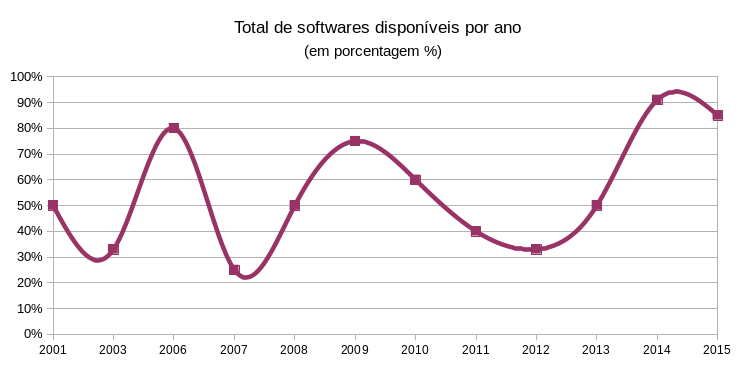
\includegraphics[scale=0.65]{imagens/softwares-disponivel-por-ano.png}
  \caption{Gráfico em linha com o total de softwares disponíveis por ano}
  \label{softwares-disponivel-por-ano}
\end{figure}

A Figura \ref{softwares-disponivel-por-ano} apresenta em cada ano quantos
porcentos do total de softwares publicados com indicação de fonte estão ainda continuam
disponíveis hoje, ou seja, quantos qual é a taxa de softwares que continuam
disponíveis hoje dentro do conjunto de softwares publicados em cada ano com
informação sobre fonte para download.  Os anos de 2002, 2004, 2005, e
anteriores a 2001 não possuem softwares publicados com fonte indicada no artigo
ainda disponível, portanto não constam no gráfico suas informações.

Ao analisar a figura percebemos que há um leve crescimento na disponibilidade
dos softwares nos anos mais recentes, com isso podemos responder à nossa
questão de pesquisa {\bf Q3} (\QuestaoTres).

Existe uma leve tendência da fontes informadas, páginas web, se tornarem
indisponível ao longo do tempo, é possível notar que em 2006 80\% de todos os
softwares de análise estática publicados estão ainda disponíveis, este número
cresce em 2014 chegando a 90\%, e cai no ano seguinte para 85\%, apesar de não
estar sempre crescente, e de termos uma amostra pequena, apenas 60 softwares,
este leve indício confirma a afirmação de \citeonline{robles2010replicating}.

Esses 37 softwares com fonte disponível foram avaliados em relação ao segundo
aspecto em respeito à de que forma estão disponíveis, os artigos informam onde
obter tais softwares, os softwares estão realmente disponíveis, as fontes
indicadas foram acessadas e na presente data deste trabalho estão funcionando e
acessíveis, mas queremos saber em qual formato estes softwares estão
disponíveis?

\begin{itemize}
  \item Código fonte disponível
  \item Apenas binários disponível
\end{itemize}

Entre estes apenas 3 não possuem código fonte disponível, 34 estão com o código
fonte disponível publicamente, dentre elas 13 não informam licença alguma
apensar de ter o código fonte disponível, 21 informam licenças de FOSS ({\it
free and open source software}):

\begin{itemize}
  \item 8 usam GNU General Public License;
  \item 2 usam Apache License;
  \item 4 usam BSD License;
  \item 3 usam Eclipse Public License;
  \item 2 usam University of Illinois/NCSA Open Source License;
  \item 1 usa licença {\it FrontEndART Software Ltd}; e
  \item 1 usa licença {\it SAnToS Laboratory Open Academic License}.
\end{itemize}

Com essas informações podemos responder à terceira e última questão de
pesquisa desse estudo {\bf Q4} (\QuestaoQuatro).

Entre os 37 softwares disponíveis 21 podem ser modificados para se adaptar às
necessidades emergentes sem necessidades de solicitação prévia de autorização
aos autores originais devido ao uso de licenças livres. Os 13 softwares
restantes com código fonte disponível mas sem licença expressa podem
eventualmente serem modificados mas a falta de uma licença impõe à necessidade
de solicitar permissão aos autores originais.

35\% dos softwares disponíveis podem ser adaptados de forma incremental para
aproveitar oportunidades emergentes, 21\% podem mediante prévia autorização do
autor original serem modificados, e apenas 5\% não oferecem essa possibilidade
por não disponibilizarem o código fonte publicamente.

\section{Ameaças à validade}

Estamos considerando que o código fonte é necessário para repetir um dado
estudo mas pode ser que em alguns casos o estudo possa ser repetido mesmo sem a
disponibilidade do mesmo, isto poderia ser resolvido realizando a repetição
de cada estudo na prática e a partir daí identificar se o código fonte dos
softwares desenvolvidos são requeridos.

A escolha de um domínio de aplicação específico para seleção dos softwares
pode ser um fator de influencia nos resultados obtidos, sendo possível que
o número de artigos com publicação de softwares com código fonte disponível
encontrado não reflita nos outros domínios, os problemas diagnosticados
neste domínio pode não ser verdade em outros domínios, sendo necessário
realizar o mesmo estudo em outros domínios.

A leitura dos artigos na revisão estruturada para identificar se publicam
softwares de análise estática de código fonte, se disponibilizam fonte para
obtenção de tais softwares, e se os softwares são mesmo do domínio de aplicação
de análise estática de código fonte podem ter maior validade se feitos em
par e revisados por outros pesquisadores, neste estudo tudo foi feito pelo
autor deste estudo e não houve revisão por pesquisadores independentes.

\section{Conclusões}

Dos 346 artigos do SCAM e 1533 artigos do ASE analisados na revisão estruturada
apenas 44\% (155 artigos) e 18\% (281 artigos) continham os termos pesquisados
no filtro automático da segunda atividade da revisão, respectivamente.

Deste total apenas 11\% (41 artigos) e 4\% (62 artigos) foram selecionados na
terceira e última atividade da revisão contendo publicação de ferramenta de
análise estática.

Resultando em 103 artigos com publicação de {\it software científico} de
análise estática de código fonte, apenas 35 possuem fonte para obtenção do
software, sendo 32 de código aberto, ou seja, com disponibilidade de
código fonte, e 3 grátis, apenas binários disponível. Ou seja, apenas 31\% dos
artigos com publicação de software disponibilizam o código fonte das mesmas.
Isto significa que 69\% dos artigos com publicação de software de análise
estática de código fonte são potencialmente impossíveis de serem repetidos, já
que os artefatos originais são necessários para tal atividade e o artigo não
disponibiliza o código fonte dos mesmos.

% o artigo com resumo do RESER 2011 diz \cite{knutson2010report}:
% 4) Re-
% search tools are either not available or not usable, so precise
% replication is impractical [1, 2, 8, 18, 19].

Muitos outros aspectos podem ser levados em consideração quando se está
avaliando a capacidade de repetir ou replicar um estudo, aqui avaliamos apenas
a disponibilidade de código fonte dos softwares científicos, mas inúmeros detalhes
pormenores são necessários, tais como: indicar qual versão do software foi
utilizado no estudo, 

No entando, consideramos que nem todos os scripts e código fonte pode
valer o custo de dua publicação, sabe-se que umas das barreiras para publicação
de muitos destes artefatos são as dificldades em tal atividade,
e as objeções a tal prática de ter RR reques um esforço adicional \cite{madeyski2017would},
em muitos
estudos o simples fato de não possuir código disponível pode não levar
a problemas para alcançar a meta final que é aumento da validade do estudo,


Todas as atividades e artefatos produzidos neste estudo estão documentados em
repositório público no
Github\footnote{\url{http://github.com/joenio/dissertacao-ufba-2016}}, o
Apêndice \ref{apendice-revisao-estruturada} traz mais informações.

%, uma lista completa e
%o endereço de cada edição onde os artigos foram obtidos está documentado no
%Apêndice \ref{edicoes-conferencias}


\section{Análise da complexidade estrutural dos softwares científicos}

Análise da complexidade estrutural dos softwares científicos de análise
estática de código-fonte como forma de avaliar a qualidade interna dos mesmos.

\label{complexidade-ferramentas}

% O manifesto de Dagstuhl ao falar sobre sustentabilidade de software levanta também preocupações em relação à sua qualidade:
% 
% \begin{quote}
%   Como podemos garantir a qualidade do software acadêmico? Como podemos
%   monitorar, orientar, divulgar e avaliar a qualidade do software acadêmico?
%   Como podemos gerenciar e garantir confiança entre as equipes de pesquisa
%   acadêmica considerando software desenvolvido para métodos de presquisa e/ou
%   de produção?
% \end{quote}

% Good enough practices in scientific computing
% If you or your group are creating tens of thousands of lines of software for use by hundreds of
% people you have never met, you are doing software engineering. If you’re writing a few dozen
% lines now and again and are probably going to be their only user, you may not be doing engi-
% neering, but you can still make things easier on yourself by adopting a few key engineering
% practices. What’s more, adopting these practices will make it easier for people to understand
% and (re)use your code.
% The core realization in these practices is that being readable, reusable, and testable are all
% side effects of writing modular code, i.e., of building programs out of short, single-purpose
% functions with clearly-defined inputs and outputs [12]. Much has been written on this topic
% [12–14], and this section focuses on practices that best balance ease of use with benefit for you
% and collaborators.

Poucos estudos sobre avaliação de qualidade interna de softwares fazem isso com
{\it softwares científicos}, algo de extrema importância para compreender como
tais artefatos estão contribuindo para a divulgação do conhecimento e para
replicação dos resultados das pesquisas em engenharia de software.

Avaliar os {\it softwares científicos} do ponto de vista de sua qualidade pode
ajudar a compreender quanta atenção é dada ao seu desenvolvimento, uma vez que
tradicionalmente os seus autores enfrentam problemas com manutenabilidade
\cite{Prlic2012}.

Manutenabilidade é uma característica de qualidade externa que indica o quão
fácil é realizar atividades de evolução e manutenção em componentes de
software, ela pode ser medida através de características de qualidade interna,
uma vez que grande parte dos engenheiros de software assumem que uma boa
estrutura interna resulta em boa qualidade externa \cite{Fenton2014}. A
estrutura interna de um software pode ser avaliada através da sua complexidade,
uma característica bastante referenciada na literatura como um importante
indicador de qualidade, estudos mostram que quanto maior a complexidade, maior
é o esforço de manutenção \cite{hashim1996software, Darcy2005}, em especial a
complexidade estrutural, uma medida definida em termos de acoplamento e coesão
\cite{Terceiro2012}.

Assim temos como objetivo neste estudo avaliar a qualidade dos {\it softwares
científicos} a partir de sua complexidade estrutural.

Os softwares avaliados neste estudo serão do domínio de aplicação de análise de
código-fonte, ferramentas de análise estática de código-fonte tem sido
continuamente desenvolvidas e tem se tornado mais e mais comuns no ciclo de
desenvolvimento de software \cite{Novak2010}, e apesar da rápida e constante
evolução da área, ainda há carência de estudos avaliando estas ferramentas
\cite{Li2010}, especialmente os {\it softwares científicos}.

% referencia sobre complexidade:
% Livro: Software Metrics, A Rigorous and Practical Approach [3rd 2015]
% 9.1.1 Structural Complexity Properties
%
%
%We will also
%investigate the maintainability measures taxonomy by
%Oman et al where 92 measures are listed and classified [24].
%[24] Oman, P., Hagemeister, J., and Ash, D., A Definition
%and Taxonomy for Software Maintainability, report
%SETL Report 91-08-TR, University of Idaho, 1991.
%
%\cite{Measurements of Software Maintainability}
%
%Taxonomia, metricas, etc ... sobre manutenabilidade de software.
%
%\cite{Metrics for Assessing a Software System’s Maintainability}

\subsection{Planejamento do estudo}

Os dados serão coletados através de uma revisão estruturada, análise estática
com o Analizo, e caracterizacao manual das ferramentas a partir das fontes:
artigo, documentação, sites e repositórios da ferramenta.

Além da revisão estruturada, que será a fonte de ferramentas da academia,
iremos também buscar e selecionar ferramentas da indústria, para isto
buscaremos fontes e catálogos através de pesquisa livre na internet.

Coletamos para cada ferramenta selecionada suas métricas de código-fonte
através da execução da ferramenta {\it analizo metrics}, esta coleta foi
automatizada pelo script {\it
analyze-all-projects}\footnote{http://github.com/joenio/dissertacao-ufba-2016/blob/master/dataset/analyze-all-projects}
escrito durante este estudo disponível no
repositório\footnote{http://github.com/joenio/dissertacao-ufba-2016} desta
pesquisa.

\subsection{Analizo} \label{analizo}

Analizo é um conjunto de ferramentas para análise de código-fonte e
visualização com suporte a múltiplas linguagens de programação, software livre,
extensível e capaz de lidar com código-fonte não mais compilável. A capacidade
de lidar com código-fonte não mais compilável permite analisar código-fonte
com erros de sintaxe, com referências a bibliotecas não mais disponíveis, ou
que usem bibliotecas com mudanças de API.

%Ela será a ferramenta utilizada por nós durante este estudo para análise do
%código-fonte das ferramentas selecionadas, a decisão pela ferramenta Analizo
%se deu por conta dela ser também a escolha utilizada nos trabalhos
%relacionados (seção \ref{trabalhos-relacionados}) onde estamos nos apoiando,
%além disso, Analizo também tem sido utilizada em diversos estudos
%desenvolvidos em nosso grupo de pesquisa (seção \ref{trabalhos-analizo}).

\subsubsection{Arquitetura do Analizo}

A arquitetura do Analizo é apresentada na Figura \ref{arquitetura-analizo}
através de uma representação {\it Layered Style} \cite{Clements2002}, cada
camada no diagrama usa apenas os serviços oferecidos pela camada diretamente
abaixo dela.

\begin{figure}[h]
\center
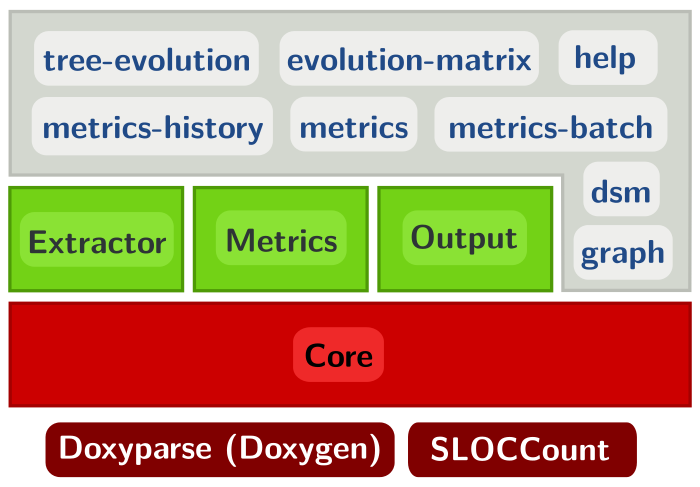
\includegraphics[scale=0.3]{imagens/analizo-architecture.png}
\caption{Arquitetura do Analizo, usando Layered Style \cite{Clements2002}}
\label{arquitetura-analizo}
\end{figure}

O {\it Core} contém as estruturas de dados usadas para armazenar informações a
respeito do código-fonte sendo analisado, lista de módulos\footnote{o
conceito ``módulo'' é usado como um termo abrangente para designar diferentes
tipos de estruturas usados em desenvolvimento de software, como classes e
arquivos fonte C}, elementos dentro de cada módulo (atributos, variáveis,
métodos, funções) e informações de dependência (chamada, herança, etc). Esta
camada implementa a maior parte da lógica de negócio do Analizo, e não depende
de nenhuma outra camada.

A camada {\it Extractor} lida com as informaçoes de código-fonte obtidas pelas
diferentes estratégias implementadas no Analizo. Os extratores obtém
informações do código-fonte e armazenam em estruturas de dados na camada {\it
Core}. Adicionar um novo extrator requer apenas a criação de uma nova subclasse
que faça interface com uma ferramenta externa ou que ela própria realize análise
de código-fonte.

%% Atualmente existem dois extratores, ambos fazem interface
%% com ferramentas externas de análise estática de código-fonte:
%% 
%% \begin{itemize}
%% 
%%   \item {\it Analizo::Extractor::Doxyparse} é uma interface para o Doxyparse,
%%   um parser de código-fonte para C, C++ e Java desenvolvida por nosso grupo de
%%   pesquisa\cite{Costa2009}. Doxyparse é baseado no
%%   Doxygen\footnote{doxygen.org}, um sistema de documentação multi-linguagem.
%% 
%%   \item {\it Analizo::Extractor::Sloccount} é uma interface para o
%%   Sloccount\footnote{dwheeler.com/sloccount} desenvolvido por David A. Wheeler,
%%   uma ferramenta que calcula o número efetivo de linhas de código.
%% 
%% \end{itemize}

A camada {\it Metrics} processa as estruturas de dados do {\it Core} para
calcular métricas, até o momento Analizo suporta um conjunto razoável de
métricas (listadas na Seção \ref{metricas}), uma representação desta camada
pode ser vista no diagrama da Figura \ref{arquitetura-metrics-analizo}.

A camada {\it Output} é responsável por lidar com diferentes formatos de
arquivos.  Atualmente, apenas o formato DOT é implementado no Analizo para
representar grafo de dependencia, adicionar novos formatos é simplesmente
adicionar novas classes nesta camada.

\begin{figure}[h]
\center
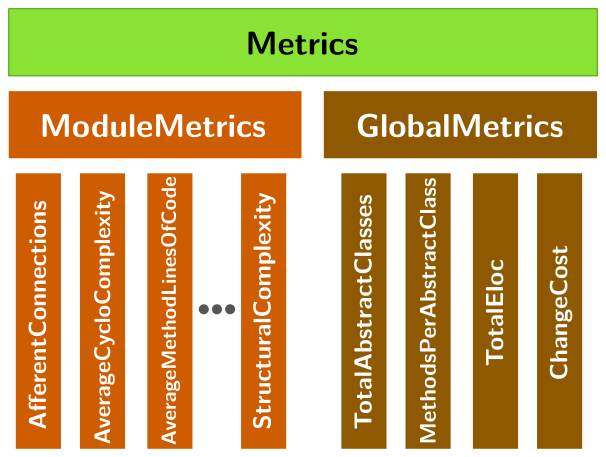
\includegraphics[scale=0.4]{imagens/analizo-metrics-architecture.png}
\caption{Arquitetura do módulo metrics em detalhes, usando Layered Style \cite{Clements2002}}
\label{arquitetura-metrics-analizo}
\end{figure}

A última camada, {\it Tools}, fornece um conjunto de ferramentas de linha de comando que
constituem a interface do analizo, tanto para usuários finais quanto para
aplicações de mais alto nível. Estas ferramentas usam serviços providos pelas
outras camadas: eles instanciam as estruturas de dados do {\it Core},
inicializam um ou mais extratores, opcionalmente executam o processador de
métricas, instanciam um módulo de formato de saída, e gerencia todos eles para
prover o resultado desejado. A maioria das funcionalidades descritas na Seção
\ref{funcionalidades} são implementadas nesta camada.

Estas ferramentas são pensadas na filosofia UNIX: fazem uma tarefa
especializada e geram uma saída que pode ser utilizada como entrada para outras
ferramentas, seja para o próprio Analizo ou para ferramentas externas. Algumas
das ferramentas implementadas no Analizo são feitas consumindo saída gerada por
outra ferramenta, outras são desenhadas para prover saída em formato específico
para aplicações externas, por exemplo, programas para desenho de grafos ou
visualização de dados.

\subsubsection{Funcionalidades}\label{funcionalidades}

\begin{itemize}

\item {\bf Análise de código-fonte multi-linguagem}

Atualmente Analizo suporta análise de código-fonte escrito em C, C++ e Java.
Entretanto, pode ser facilmente estendido para suportar outras linguagens pois
pode potencialmente suportar as inúmeras outras linguagens suportadas pelo Doxygen.

\item {\bf Métricas}\label{metricas}

O Analizo suporta tanto métricas em nível de projeto, que é calculada para todo o projeto,
quanto métricas em nível de módulos, que é calculado individualmente para cada módulo.
No nível de projeto, Analizo também provê estatística descritiva básica para cada métrica em
nível de módulo: soma, média, mediana, moda, desvio padrão, variância, skewness e kurtosis da
distribuição, valores mínimo e maximo. As seguintes métricas são suportadas até o momento:

\begin{itemize}

  \item Métricas em nível de projeto: Change Cost, Total Abstract Classes,
  Total Coupling Factor, Total Effective Lines of Code, Total Lines of Code,
  Methods per Abstract Class, Total Number of Modules, Total number of modules
  with at least one defined attributes, Total number of modules with at least
  one defined method, Total Number of Methods.

  \item Métricas em nível de módulo: Afferent Connections per Class, Average
  Cyclomatic Complexity per Method, Average Method Lines of Code, Argument with
  'nonnull' attribute passed null, Average Number of Parameters per Method,
  Allocator sizeof operand mismatch, Assigned value is garbage or undefined,
  Bad deallocator, Bad free, Coupling Between Objects, Dead assignment,
  Divisions by zero, Double free, Depth of Inheritance Tree, Dereference of
  null pointer, Dereference of undefined pointer value, Potential buffer
  overflow in call to 'gets', Lack of Cohesion of Methods, Lines of Code,
  Memory leak, Max Method LOC, Number of Attributes, Number of Children, Number
  of Methods, Number of Public Attributes, Number of Public Methods,
  Out-of-bound array access, Offset free, Potential insecure temporary file in
  call 'mktemp', Response for a Class, Result of operation is garbage or
  undefined, Return of stack variable address, Stack address stored into global
  variable, Structural Complexity, Undefined allocation of 0 bytes,
  Use-after-free, Uninitialized argument value.

\end{itemize}

É possível especificar que certos diretórios dentro do projeto não devem ser
analisados, de forma que o Analizo ignore tais arquivos durante a análise e o
cálculo de métricas.

\item {\bf Processamento em lote}\label{lote}

A maioria dos estudos quantitativos em engenharia de software envolve aquisição
de métricas de código-fonte de um grande número de projetos, processar cada
projeto individualmente é pouco prático, passível de erros e difícil de
repetir. Analizo pode processar multiplos projetos em lote e produzir arquivo
de dados CSV com métricas de cada projeto, bem como um resumo com as métricas
em nível de projeto de todos os projetos. Estes arquivos de dados podem ser
facilmente importados em ferramentas de estatística ou planilhas para análise
futura. Esta capacidade de processar em lote pode também ser utilizada para
analisar várias versões de um mesmo projeto, especialmente útil em estudos
sobre evolução de software.

%% Este processamento em lote pode se beneficiar de processamento paralelo dando
%% mais agilidade e na análise e reduzindo o tempo total de processamento.  A
%% saída pode ser também escrita diretamente em um banco de dados relacional ao
%% invés de gerar arquivos CSV. Outro recurso voltado à performance é um sistema
%% de cache para as informações previamente calculadas, evitando repetição de
%% processamento.

\item {\bf Histórico de métricas}

Algumas vezes pesquisadores precisam processar o histórico de projetos de
software de uma forma mais escalável. Analizo pode processar repositórios de
controle de versão e prover arquivo de dados CSV com valores de métricas para
cada revisão onde o código-fonte foi alterado no projeto, ou pode também gravar
os valores diretamente num banco de dados ao invés de usar arquivos CSV. Repositórios Git e
Subversion são suportados diretamente, repositórios CVS devem ser convertidos
para Git de forma manual.

\item {\bf Grafo de dependência}

Analizo pode gerar saída com informações sobre dependência entre as entidades
do projeto em um formato adequado para processamento por ferramentas de
renderização de grafos do Graphviz\footnote{graphviz.org}. A Figura
\ref{sample-graph} apresenta um exemplo de grafo desenhado pela ferramenta {\it
dot} do Graphviz a partir da saída gerada pelo Analizo {\it graph}.

\begin{figure}[h]
\center
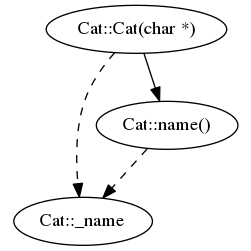
\includegraphics[scale=0.4]{imagens/sample-graph.png}
\caption{Exemplo de grafo de dependência}
\label{sample-graph}
\end{figure}

%% \item {\bf Matriz de evolução}
%% 
%% Outra funcionalidade útil do Analizo é a visualização de matrizes de evolução
%% \cite{Lanza2001}. Ao processar cada release de um projeto (ver Seção
%% \ref{lote}), o usuário pode solicitar a criação de uma matriz de evolução a
%% partir de arquivos de dados individuais. A Figura \ref{sample-evolution-matrix}
%% apresenta um exemplo de uma matriz produzida pelo Analizo.
%% 
%% \begin{figure}[h]
%% \center
%% 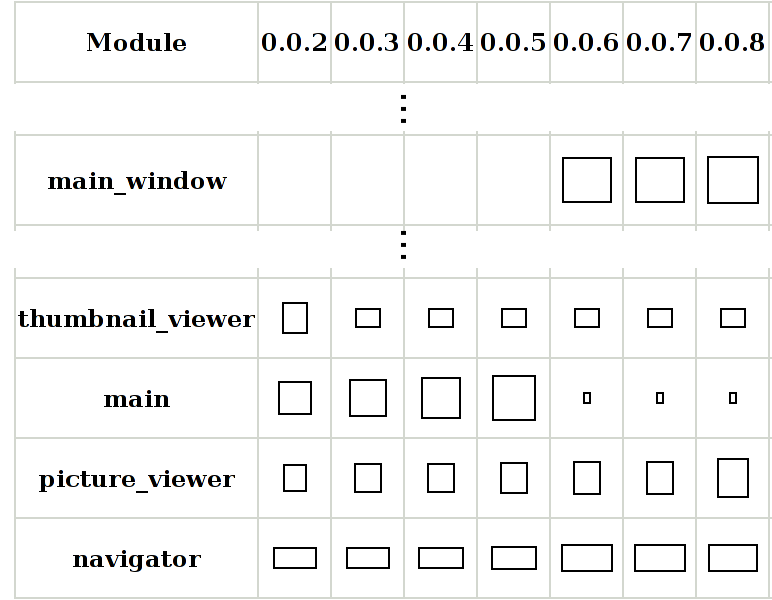
\includegraphics[scale=0.2]{imagens/sample-evolution-matrix.png}
%% \caption{Exemplo de matriz de evolução}
%% \label{sample-evolution-matrix}
%% \end{figure}
%% 
%% \item {\bf Matriz de estrutura de projeto}
%% 
%% Uma funcionalidade recente do Analizo é a representação visual do
%% relacionamento entre os módulos do projeto em forma de uma matriz de estrutura
%% de projeto ({\it Design Structure Matrix}) \cite{Maccormack2006}, uma DSM é a
%% representação de um grafo de dependência em forma de uma matriz quadrada. Um
%% exemplo gerado pelo Analizo pode ser visto na Figura \ref{sample-dsm}.
%% 
%% \begin{figure}[h]
%% \center
%% 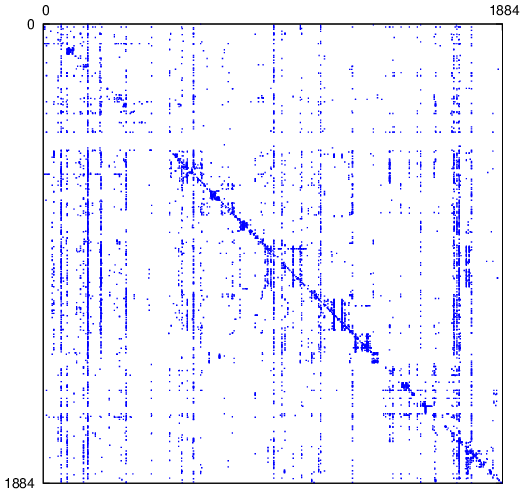
\includegraphics[scale=0.3]{imagens/sample-dsm.png}
%% \caption{Exemplo de matriz de estrutura de projeto}
%% \label{sample-dsm}
%% \end{figure}

\end{itemize}

\subsubsection{Uso em trabalhos de pesquisa}
\label{trabalhos-analizo}

Analizo tem sido extensivamente usado por nosso grupo de pesquisa em diversos
estudos:

\begin{itemize}

  \item \cite{Amaral2009} usou o grafo de dependencia gerado pelo Analizo para
  gerar uma matriz de evolução em um estudo de caso com o projeto VLC.

  \item \cite{Costa2009} fez uma comparação entre diferentes estratégias para
  extração de informação de dependencias entre módulos do código-fonte,
  resultando no desenvolvimento do Doxyparse - o extrator baseado no Doxygen do
  Analizo.

  \item \cite{Terceiro2009} usou métricas em um estudo exploratório sobre a
  evolução da complexidade estrutural em projetos de software livre escritos em
  C.

  \item \cite{Morais2009} usou a ferramenta de métricas do Analizo como backend
  para o Kalibro, um software para avaliação e observação de métricas de código-fonte.
  
  \item \cite{Terceiro2010} usou o processamento de histórico de métricas para
  realizar um estudo exploratório sobre a evolução da complexidade estrutural em
  7 projetos de servidor web de diferentes tamanhos.

  \item \cite{Meirelles2010} usou o processamento em lote do Analizo para
  processas o código-fonte de mais de 6000 projetos de software livre do
  repositório Sourceforge.net.

  \item \cite{Meirelles2011} usou o Analizo em um estudo sobre impacto de
  métricas de código-fonte na atratividade de projetos de softwares livres.

  \item \cite{Terceiro2012Understanding} usou o Analizo para investigar fatores
  que influenciam na evolução da complexidade estrutural em projetos de software
  livres.

  \item \cite{Silva2012} usou o Analizo para minerar 16000 revisões de
  repositórios de projetos de software para investigar o potencial de uma nova
  métrica chamada Lack of Concern-based Cohesion.

  \item \cite{Ronaldo2015} utilizou o Analizo para extrair métricas de
  código-fonte de 14 versões do sistema Android e estudar a evoluçao da API e
  seus aplicativos.

\end{itemize}

A maioria destes trabalhos contribuíram com melhorias para o Analizo, fazendo
dele uma ferramenta bastante apropriada para pesquisas envolvendo análise de código-fonte,
sendo útil tanto para pesquisadores trabalhando com análise de código-fonte
quanto para profissionais que precisam analisar seus projetos em busca de
potenciais problemas ou melhorias.

Analizo é software livre, distribuído sob a licença GNU General Public License
versão 3. Seu código-fonte, bem como pacotes binários, manuais e tutoriais
podem ser obtidos em \url{http://www.analizo.org}. Todas as ferramentas são
auto-documentadas e podem ser consultadas como páginas de manual UNIX. Analizo
é escrito em Perl, sua última versão 1.19.1 lançada em 01 de Setembro de 2016
será a versão utilizada neste estudo.

\section{Análise dos dados} \label{analise}

Os dados coletados incluem a caracterização das ferramentas de análise
estática, bem como, os valores das métricas de código-fonte de complexidade
estrutural para cada ferramenta. A coleta das métricas de
código-fonte será realizada pelo Analizo com o auxílio do script {\em
analyze-all-projects}\footnote{http://github.com/joenio/dissertacao-ufba-2016/blob/master/dataset/analyze-all-projects},
escrito durante o desenvolvimento deste estudo. A caracterização será feita a
partir dos artigos selecionados na revisão estruturada, documentação, site do
projeto e repositório das ferramentas.

Todos os dados serão agregados numa planilha, a análise exploratória será
realizada comparando pares de ferramentas de tamanhos similares, o tamanho das
ferramentas será dado pelo número de módulos. O tamanho deve ser
levado em conta pois sabe-se que ele influencia nos valores de métricas de
código-fonte, complexidade estrutural, por exemplo, sofrem
de tal infuência.

Outro fator de grande influência é o domínio de aplicação, como estamos
estudando apenas ferramentas de análise estática, considera-se que este fator
está isolado e não sofreremos sua influência.

Uma vez que tenhamos o conjunto de pares de ferramentas de tamanhos similares
iremos analisar os valores das métricas de complexidade estrutural e custo de
mudança para cada par e interpretar qual das ferramentas possui melhor
manutenabilidade, partimos do princípio que valores menores para cada uma
destas métricas implicam em melhor manutenabilidade.

Esta análise dos pares irá apenas nos dizer quais ferramentas tem melhor
manutenabilidade em comparação com as demais, não é uma informação que
pode ser interpretada de forma geral, ela não diz que a ferramenta tem
ou não uma boa manutenabilidade, indica apenas que uma certa ferramenta
tem melhor manutenabilidade que uma outra.

Com o conhecimento de quais ferramentas tem melhor manutenabilidade iremos
utilizar as dimensões caracterizadas para cada ferramenta para verificar se
tais características influenciam na manutenabilidade, não apenas notar se
influenciam, mas poderemos notar quais características influenciam. Por
exemplo, será que as ferramentas que aceitam como entrada análise da linguagem
Java possuem melhor manutenabilidade do que aquelas que aceitam C++?

Assim, iremos analisar e interpretar cada par de ferramenta de tamanho
similar, sempre à luz de suas características a fim de compreender quais
características influenciam em sua manutenabilidade.

Com isso temos 11 projetos, destes iremos analisar longitudalmente
as releases e a evolucao dos valores de SC e CC (Change Cost), sao elas:

WALA                     13 releases
error-prone              13 releases
JastAdd                  13 releases
SPARTA                   13 releases
Indus                    (poucos releases, deixando fora da analise longitudinal)
Kiasan/Bogor             (mudou a forma de distribuir ao longo dos releases, dificil obter de forma consistente as versoes)
Lotrack                  (sem releases, poucos commits no github, apenas 11)
PtYasm                   (nao tem releases disponivel, apenas a ultima versao)
srcML                    (releases nao encontrado)
GumTree                  (tem apenas 2 releases do repositorio github)
Sonar Qube Plug-in       (apenas 4 releases no github)
CIVL                     13 releases
CodeBoost                (poucos releases, apenas 6 versoes para download no site)
2LS                      (poucos releases, apenas 7)

% aproveitar perte destas referencias ao justificar o uso de percentis ao inves de média
%
%Observar métricas de código-fonte em nível de projetos de software leva
%ao seguinte desafio: como obter valores de métricas que representem todo o projeto sendo
%que métricas de código-fonte usualmente são calculadas para cada elemento do sistema, como arquivos ou classes?
%
%Este desafio tem sido amplamente discutido em estudos sobre definição de
%intervalos de referência ({\it thresholds}) para métricas de
%código-fonte \cite{Shatnawi2010, Kaur2013, Herbold2011}. Intervalos de
%referência são valores conhecidos para uma dada medida
%\cite[Chapter~2.1]{Lanza2007} com algum valor semantico, por exemplo, se
%medirmos a altura das pessoas e definirmos até 2 metros como alto, então
%pessoas acima de 2 metros serão classificadas como muito altas.
%
%Intervalos de referência podem ser definidos de diversas formas, desde
%abordagens baseadas em modelos estatísticos \cite{Shatnawi2010, Kaur2013}
%até aprendizado de máquina \cite{Herbold2011} e inteligência artificial.
%Entre as inúmeras abordagens, muitas partem de estudos empíricos
%usando softwares da indústria como objeto de estudo, geralmente com
%softwares de domínios específicos, parte-se da coleta de dados de
%métricas de código-fonte e com uso de uma abordagem, ou uma combinação entre
%elas, chega-se aos intervalos.
%
%Estes intervalos são também continuamente avaliados a fim de saber se são
%válidos ou não, as abordagens utilizadas para calcular os intervalos levam em
%consideração inúmeros aspectos na tentativa de validar os valores encontrados,
%como por exemplo a natureza dos dados, se seguem a lei de distribuição de
%potência
%\cite{Wheeldon2003,Potanin2005,Concas2007,Ferreira2009,Yao2009,Clauset2009} ou
%seguem uma distribuição normal
%\cite{Baxter2006,Lanza2007,Herraiz2011,Herraiz2012}, avaliam ainda se possuem
%cauda longa, se são livre de escala, entre outros aspectos.

\section{Resultados}

(pendente)

\section{Ameaças à validade}

(pendente)

\section{Conclusões}

(pendente)

%% usar a dimensao abaixo para definir quais usar na avaliacao longitudinal:
%% 
%% %, e qual a frequência de lançamentos indicando se são
%% %atualizadas frequentemente ou estão obsoletas.
%% 
%% \begin{description}
%% 
%%   \item {\it Lançamentos ({\it Releases}) - quantos lançamentos por ano:}
%%     \begin{itemize}
%%       \item Frequentemente $>=$ 3 vezes ao ano\\
%%         {\it \small novas versões da ferramenta são lançadas 3 ou mais vezes por ano}
%%       \item Ocasionalmente $<$ 3 vezes ao ano\\
%%         {\it \small novas versões da ferramenta são lançadas menos que 3 vezes ao ano}
%%       \item Obsoleta 0 vezes ao ano\\
%%         {\it \small intervalo entre novos lançamentos é maior que 1 ano}
%%     \end{itemize}
%% 
%% \end{description}
%% 
%% O autor não deixa claro como categorizar softwares sem lançamentos nos últimos
%% anos mas com histórico de lançamento frequente em anos anteriores. Assim, será
%% considerado todo o histórico de lançamentos e só serão considerados obsoletos
%% por exemplo softwares que nunca tenha tido mais de 1 lançamento ao ano
%% considerando todo o histórico dele. Da mesma forma, será considerado ocasional
%% apenas aqueles que sempre tiveram no máximo 2 lançamentos ao ano. Esta dimensão
%% irá nos dizer o grau de evolução de cada ferramenta, considerando que softwares
%% com lançamentos frequentes estão evoluindo.
%% 
%% ======================
%% 
%% \begin{description}
%% 
%%   \item {\it Entrada - quais tipos de arquivos podem ser carregados na ferramenta:}
%%     \begin{itemize}
%%       \item Código-fonte - arquivos de código texto podem ser carregados
%%       \item Byte code - arquivos com Java Byte Code ou Microsoft
%%       \item Linguagem intermediária (MSIL) pode ser carregada
%%     \end{itemize}
%% 
%%   \item {\it Linguagens suportadas - quais linguagens de programação a ferramenta suporta:}
%%     \begin{itemize}
%%       \item .NET - todas as linguagens compiladas em bibliotecas ou programas no framework .NET
%%       \item VB .NET - suporta VB.NET
%%       \item C\# - suporta C\#
%%       \item Java - suporta linguagem de programação Java
%%       \item C, C++ - suporta linguagem de programação C ou C++
%%     \end{itemize}
%% 
%% \end{description}
%% 
%% As dimensões apresentada por \citeonline{Novak2010} não cobrem alguns aspectos
%% importantes percebidos ao longo deste estudo, assim novas dimensões serão utilizadas
%% em complemento às dimensões citadas acima.
%% 
%% \begin{description}
%% 
%%   \item {\it Linguagem de programação - em que linguagem de programação à ferramenta é escrita:}
%%     \begin{itemize}
%%       \item .NET
%%       \item VB .NET
%%       \item C\#
%%       \item Java
%%       \item C, C++
%%     \end{itemize}
%% 
%% \end{description}
%% 
%% 
%% ================
%% 
%% 
%% A ferramenta livre {\it sloccount}\footnote{http://www.dwheeler.com/sloccount}
%% foi utilizada para identificar a linguagem de programação em que cada
%% ferramenta é implementada. O tamanho em número de classes foi extraído utilizando a ferramenta
%% Analizo, uma das inúmeras métricas que ela extraí é a contagem do número total
%% de classes de um sistema. 
%% 
%% ===============
%% 
%% \section{Data collection procedure}
%% 
%% \begin{itemize}
%%   \item Pesquisa livre em fontes na internet para busca e seleção de ferramentas da indústria
%%   \item Obtenção do código-fonte de cada ferramenta
%%   \item Cálculo e coleta de métricas de código-fonte
%%   \item Obtenção de código-fonte de mais versões de ferramentas com {\it Lançamentos} frequentes ou ocasionais
%%   \item Cálculo e coleta de métricas de código-fonte das novas versões
%% \end{itemize}
%% 
%% ==============
%% 
%% \subsection{Analizo}
%% 
%% Numa primeira análise dos valores coletados pelo Analizo notamos uma anomalia
%% nos valores da métrica CBO, o que nos levou a investigar de perto os motivos,
%% esta anomalia se apresentava como valores extremamente altos para esta métrica,
%% bastante discrepante com as demais métricas calculadas.
%% 
%% Para entender se estes valores estavam corretor ou não, utilizamos uma outra
%% ferramenta para cálculo das métricas, em nossos estudos encontramos e
%% utilizamos uma versão de avaliação da ferramenta {\it SciTools
%% Understand}\footnote{http://scitools.com/trial-download-3} em sua versão
%% ``4.0.853'' em Linux 64 bits. Os dados extraídos por esta ferramenta podem ser
%% encontrados em nosso
%% repositório\footnote{http://github.com/joenio/dissertacao-ufba-2016/tree/master/dataset/Understand
%% SciTools}. Eles demonstraram que os valores calculados pelo Analizo estavam
%% bastante alto em comparação com as demais métricas.
%% 
%% Assim, descobrimos que o Analizo tinha de fato um erro no cálculo da métrica
%% CBO, erro que foi corrigido durante este estudo e disponibilizado na versão
%% mais recente do Analizo, versão que está sendo utilizada aqui.
%% 
%% 
%% =============
%% 
%% \subsection{Ferramentas da indústria}
%% 
%% Em paralelo à revisão estruturada para seleção de ferramentas da academia
%% foi realizada uma seleção manual no catálogo de ferramentas de análise estática do projeto
%% SAMATE\footnote{https://samate.nist.gov/index.php/Source\_Code\_Security\_Analyzers.html}
%% em busca de ferramentas da indústria.
%% 
%% O projeto SAMATE\footnote{http://samate.nist.gov} - {\em Software Assurance
%% Metrics and Tool Evaluation}, um projeto do NIST\footnote{http://nist.gov}
%% dedicado ao desenvolvimento de métodos que permitam avaliar e medir a
%% eficiência de ferramentas e técnicas sobre garantia de qualidade em software.
%% O site do projeto, disponível em \citeonline{SamateAnalysers}, mantém uma lista
%% de ferramentas de análise estática.
%% 
%% Nesta busca por ferramentas da indústria encontramos um total de 54 ferramentas
%% presentes no catálogo do projeto SAMATE, 19 tinham código-fonte disponível,
%% destas apenas 14 eram suportadas pelo Analizo (escritas em C, C++ ou Java).
%% 
%% Após download do código-fonte de cada ferramenta selecionada, em sua versão
%% mais recente, a ferramenta Analizo será utilizada para a coleta das métricas. 
%% A Tabela \ref{total-de-ferramentas} traz um resum com todas as ferramentas
%% selecionadas, tando da indústria quanto da academia.
%% 
%% =====
%% 
%% Deste total de 35, 4 tem lançamentos frequentes, 9 são obsoletas, 8 tem
%% lançamentos ocasional e 14 não possui informação sobre lançamentos.
%% 
%% =====
%% 
%% Uma vez identificados os artigos que publicaram ferramentas do domínio
%% desejado, procuramos no próprio artigo por referências de onde encontrar o
%% código-fonte da ferramenta. Neste momento, pode-se enfrentar algumas situações.
%% 
%% \begin{itemize}
%% 
%%   \item Os autores afirmam que a ferramenta está disponível mas o artigo
%%     não contém referências de onde encontrar o código-fonte, estes
%%     autores serão contactados, por email, solicitando informações de onde
%%     obter o código-fonte da ferramenta.
%% 
%%   \item O artigo indica onde obter o código-fonte da ferramenta, mas o acesso ao local
%%     indicado não está disponível, ou está disponível mas o software não se
%%     encontra lá, os autores serão contactados, solicitando informações
%%     atualizadas de onde obter uma cópia do código-fonte da ferramenta.
%% 
%%   \item Artigos que indicam onde obter o código-fonte da ferramenta e a referência
%%     está correta. Será feito o download do código-fonte da última versão
%%     disponível.
%% 
%% \end{itemize}
%% 
%% Uma vez que os autores sejam contactados por email e respondam com informações
%% sobre onde obter o software, a ferramenta é adicionada ao conjunto de
%% ferramentas a serem analisadas.
%% 
%% =================
%% 
%% 
%% \begin{description}
%% 
%%   \item {\it Contexto - onde a ferramenta surgiu:}
%%     \begin{itemize}
%%       \item Academia - foi desenvolvida inicialmente em contexto acadêmico
%%       \item Indústria - foi desenvolvido fora da academia
%%     \end{itemize}
%% 
%%   \item {\it Tamanho em número de classes - número de classes/módulos da ferramenta}
%% 
%%   \item {\it Nível de manutenabilidade - interpretação das seguintes métricas de código-fonte:}
%%     \begin{itemize}
%%       \item Complexidade Estrutural
%%       \item Custo de Mudança
%%     \end{itemize}
%% 
%% \end{description}
%% 
%% 
%% \subsection{Ferramentas da indústria}
%% 
%% Em paralelo à revisão estruturada para seleção de ferramentas da academia será
%% realizada uma seleção manual não estruturada para busca de ferramentas da
%% indústria. O objetivo é aumentar o conjunto de objetos de estudo bem como ter
%% ferramentas de outros contextos além da academia, isto irá proporcionar uma
%% nova dimensão na caracterzação das ferramentas e permitirá realizar comparação
%% entre ferramentas de contextos distintos.
%% 
%% 
%% ==============================
%% 
%% Dentre estas ferramentas as seguintes foram selecionadas para análise evolutiva:
%% 
%% \begin{itemize}
%%   \item Closure Compiler         
%%   \item FindBugs                 
%%   \item PMD                      
%%   \item WALA                    
%%   \item error-prone
%%   \item JastAdd
%%   \item SPARTA
%%   \item Cppcheck
%%   \item FindSecurityBugs
%%   \item Smatch
%% \end{itemize}
%% 
%% o clang foi removido pois a analise dele demorou muito, ficou rodando 1 semana q não
%% terminou, o analizo metrics que demorou tanto assim.
%% 
%% \begin{table}[H]
%% \caption{Métricas da ferramenta PMD}
%%   \centering
%% \begin{tabular}{|l|r|r|r|r|r|}
%% \hline
%% \multicolumn{1}{|c|}{\textbf{Release}} & \multicolumn{1}{c|}{\textbf{Classes}} & \multicolumn{1}{c|}{\textbf{CC}} & \multicolumn{1}{c|}{\textbf{SC 75}} & \multicolumn{1}{c|}{\textbf{SC 90}} & \multicolumn{1}{c|}{\textbf{SC 95}} \\ \hline
%% 4.2.5 & 844 & 0,06 & 6 & 15 & 28 \\ \hline
%% 4.3 & 852 & 0,06 & 6 & 15 & 28 \\ \hline
%% 5.0.0 & 1043 & 0,03 & 6 & 14 & 25 \\ \hline
%% 5.0.4 & 1052 & 0,02 & 6 & 12 & 24 \\ \hline
%% 5.1.0 & 1238 & 0,02 & 6 & 12 & 24 \\ \hline
%% 5.1.3 & 1254 & 0,02 & 6 & 12 & 25 \\ \hline
%% 5.2.0 & 1295 & 0,02 & 6 & 12 & 25 \\ \hline
%% 5.3.0 & 1341 & 0,01 & 6 & 12 & 25 \\ \hline
%% 5.3.3 & 1342 & 0,02 & 6 & 12 & 25 \\ \hline
%% 5.3.7 & 1374 & 0,01 & 6 & 12 & 25 \\ \hline
%% 5.4.0 & 1332 & 0,02 & 6 & 12 & 26 \\ \hline
%% 5.4.2 & 1366 & 0,02 & 6 & 12 & 26 \\ \hline
%% 5.5.2 & 1530 & 0,01 & 6 & 12 & 25 \\ \hline
%% \multicolumn{6}{l}{\texttt{Notas:}} \\
%% \multicolumn{6}{l}{\texttt{CC = Custo de mudança}} \\
%% \multicolumn{6}{l}{\texttt{SC = Complexidade estrutural}} \\ \hline
%% \end{tabular}
%% \label{metricas-pmd}
%% \end{table}
%% 
%% \begin{table}[H]
%% \caption{Métricas da ferramenta WALA}
%%   \centering
%% \begin{tabular}{|l|r|r|r|r|r|}
%% \hline
%% \multicolumn{1}{|c|}{\textbf{Release}} & \multicolumn{1}{c|}{\textbf{Classes}} & \multicolumn{1}{c|}{\textbf{CC}} & \multicolumn{1}{c|}{\textbf{SC 75}} & \multicolumn{1}{c|}{\textbf{SC 90}} & \multicolumn{1}{c|}{\textbf{SC 95}} \\ \hline
%% 1.0 & 1223 & 0,02 & 8 & 27 & 45 \\ \hline
%% 1.0.02 & 1685 & 0,02 & 8 & 25 & 48 \\ \hline
%% 1.1 & 1872 & 0,02 & 7 & 24 & 48 \\ \hline
%% 1.1.2 & 1720 & 0,02 & 8 & 24 & 50 \\ \hline
%% 1.2 & 1734 & 0,02 & 7 & 25 & 49 \\ \hline
%% 1.2.1.1 & 1901 & 0,02 & 6 & 24 & 48 \\ \hline
%% 1.2.2 & 1903 & 0,02 & 6 & 24 & 48 \\ \hline
%% 1.3 & 1945 & 0,02 & 6 & 24 & 52 \\ \hline
%% 1.3.3 & 2092 & 0,01 & 6 & 24 & 50 \\ \hline
%% 1.3.5 & 2143 & 0,02 & 6 & 22 & 49 \\ \hline
%% 1.3.6 & 2154 & 0,02 & 6 & 22 & 49 \\ \hline
%% 1.3.8 & 2626 & 0,02 & 7 & 24 & 54 \\ \hline
%% 1.3.9 & 2636 & 0,02 & 7 & 24 & 54 \\ \hline
%% \multicolumn{6}{l}{\texttt{Notas:}} \\
%% \multicolumn{6}{l}{\texttt{CC = Custo de mudança}} \\
%% \multicolumn{6}{l}{\texttt{SC = Complexidade estrutural}} \\ \hline
%% \end{tabular}
%% \label{metricas-wala}
%% \end{table}
%% 
%% \begin{table}[H]
%% \caption{Métricas da ferramenta FindBugs}
%%   \centering
%% \begin{tabular}{|l|r|r|r|r|r|}
%% \hline
%% \multicolumn{1}{|c|}{\textbf{Release}} & \multicolumn{1}{c|}{\textbf{Classes}} & \multicolumn{1}{c|}{\textbf{CC}} & \multicolumn{1}{c|}{\textbf{SC 75}} & \multicolumn{1}{c|}{\textbf{SC 90}} & \multicolumn{1}{c|}{\textbf{SC 95}} \\ \hline
%% 1.2.1 & 1044 & 0,05 & 7 & 20 & 36 \\ \hline
%% 1.3.4 & 1216 & 0,06 & 7 & 21 & 42 \\ \hline
%% 1.3.5 & 1257 & 0,05 & 7 & 21 & 40 \\ \hline
%% 1.3.6 & 1258 & 0,05 & 8 & 21 & 42 \\ \hline
%% 1.3.7 & 1261 & 0,05 & 7 & 22 & 42 \\ \hline
%% 1.3.8 & 1275 & 0,05 & 7 & 22 & 42 \\ \hline
%% 1.3.9 & 1354 & 0,06 & 7 & 24 & 48 \\ \hline
%% 2.0.0 & 1459 & 0,06 & 7 & 24 & 52 \\ \hline
%% 2.0.1 & 1465 & 0,06 & 7 & 24 & 54 \\ \hline
%% 2.0.2 & 1469 & 0,06 & 7 & 24 & 56 \\ \hline
%% 2.0.3 & 1489 & 0,06 & 7 & 24 & 56 \\ \hline
%% 3.0.0 & 1438 & 0,07 & 7 & 24 & 56 \\ \hline
%% 3.0.1 & 1486 & 0,07 & 8 & 25 & 56 \\ \hline
%% \multicolumn{6}{l}{\texttt{Notas:}} \\
%% \multicolumn{6}{l}{\texttt{CC = Custo de mudança}} \\
%% \multicolumn{6}{l}{\texttt{SC = Complexidade estrutural}} \\ \hline
%% \end{tabular}
%% \label{metricas-findbugs}
%% \end{table}
%% 
%% \begin{table}[H]
%% \caption{Métricas da ferramenta Closure Compiler}
%%   \centering
%% \begin{tabular}{|l|r|r|r|r|r|}
%% \hline
%% \multicolumn{1}{|c|}{\textbf{Release}} & \multicolumn{1}{c|}{\textbf{Classes}} & \multicolumn{1}{c|}{\textbf{CC}} & \multicolumn{1}{c|}{\textbf{SC 75}} & \multicolumn{1}{c|}{\textbf{SC 90}} & \multicolumn{1}{c|}{\textbf{SC 95}} \\ \hline
%% 20110119 & 1122 & 0,05 & 4 & 17 & 42 \\ \hline
%% 20110811 & 1730 & 0,1 & 5 & 20 & 40 \\ \hline
%% 20120305 & 1802 & 0,1 & 5 & 20 & 42 \\ \hline
%% 20120917 & 1836 & 0,1 & 6 & 20 & 42 \\ \hline
%% 20130227 & 1759 & 0,11 & 6 & 20 & 48 \\ \hline
%% 20130722 & 1806 & 0,1 & 6 & 20 & 48 \\ \hline
%% 20140110 & 2004 & 0,08 & 5 & 20 & 45 \\ \hline
%% 20140730 & 1573 & 0,04 & 4 & 20 & 48 \\ \hline
%% 20150126 & 1596 & 0,04 & 5 & 22 & 56 \\ \hline
%% 20150729 & 1649 & 0,04 & 6 & 26 & 65 \\ \hline
%% 20160125 & 1724 & 0,04 & 5 & 28 & 68 \\ \hline
%% 20160713 & 1860 & 0,04 & 6 & 30 & 70 \\ \hline
%% \multicolumn{6}{l}{\texttt{Notas:}} \\
%% \multicolumn{6}{l}{\texttt{CC = Custo de mudança}} \\
%% \multicolumn{6}{l}{\texttt{SC = Complexidade estrutural}} \\ \hline
%% \end{tabular}
%% \label{metricas-closurecompiler}
%% \end{table}
%% 
%% As ferramentas com poucas linhas de código foram excluidas, estas
%% apreentam Change Cost alto, já é conhecido que a definição desta métrica
%% sofre deste problema, apresenta valores altos em projetos muito pequenos,
%% tambem removemos da analise aquelas ferramentas que nao tiveram valor
%% no percentil 75\%, pois a comparacao e analise se dará neste percentil
%% principalmente.
%% 

%% Com isso temos 11 projetos, destes iremos analisar longitudalmente
%% as releases e a evolucao dos valores de SC e CC (Change Cost), sao elas:
%% Industria:
%%  FindBugs                 13 releases
%%  Closure Compiler         13 releases analisados
%%  PMD                      13 releases
%%  Smatch                   13 releases
%%  FindSecurityBugs         13 releases
%%  Cppcheck                 13 releases
%%  Splint                   (nao encontrado releases)
%%  WAP                      (apenas 7 releases no site, estou selecionando os que tenham ao menos 13 releases)

%% 
%% Comparacao entre ferramentas de tamanho similar:
%% 
%% nas 5 comparações de versões distintas com tamanhos similares entre pmd e findbugs,
%% apresentaram o mesmo resultado, pmd tem valores menos tanto para CC quanto para SC,
%% indicando que pmd tem um design mais modular que findbugs.
%% 
%% pmd 5.0.0 < findbugs 1.2.1
%% pmd 5.0.4 < findbugs 1.2.1
%% pmd 5.1.3 < findbugs 1.3.5
%% pmd 5.2.0 < findbugs 1.3.8
%% pmd 5.3.3 < findbugs 1.3.9
%% 
%% Ao comparar as imagens da matrix DSM dá para notar que isto reflete na matrix, 
%% pegando o findbugs 3.0.1 e o pmd 5.2.0, é possível notar na matrix que o findbugs
%% tem mais pontos nas duas diagonais da matrix, indicando dependencias ciclicar, e
%% design menos modular, enquanto o pmd concentra as dependencias na diagonal inferior
%% esquerda, indicando poucas dependencias ciclicar e um design mais modular.
%% 
%% findbugs	 findbugs-3.0.1	1486	0,07	8	25	56
%% pmd	 pmd-src-5.2.0	1295	0,02	6	12	25
%% 
%% /home/joenio/src/dissertacao-ufba-2016/dataset/static-analysis-tools/pmd/pmd-src-5.2.0.analizo.dsm.png
%% /home/joenio/src/dissertacao-ufba-2016/dataset/static-analysis-tools/findbugs/findbugs-3.0.1.analizo.dsm.png
%% 
%% accessanalysis < findsecuritybugs
%% indus < bogor
%% reassert > jflow
%% pmd-5.4.0 > pmd-5.3.0
%% pmd-5.4.2 > pmd-5.3.7
%% findbugs-3.0.1 > findbugs-2.0.3
%% pmd < closure-compiler
%% pixy > mpanalyzer
%% ejb > mpanalyzer
%% ejb > sparta
%% 
%% closure-compiler > wala
%% closure-compiler > wala
%% closure-compiler > wala
%% closure-compiler[Java] ? wala[Java]     (closure tem CC maior mas SC menor)
%% 
%% comparar linguagens diferentes não rola, sempre dá ruim, ver:
%% 
%% rats[C]        ? uno[C]                 (rats tem CC menor e SC maior)
%% cppcheck[C++]  ? wap[Java]              (cppcheck tem CC menor mas SC maior)
%% srcml[C++]     ? ptyasm[Java]           (srcml tem CC maior mas SC menor)
%% closure-compiler[Java] ? inputtracer[C] (closure tem CC menor mas SC diferentes nos percentis)
%% pmd[Java] ? srcml[C++]                  (pmd tem CC maior e SC diferentes nos percentis)
%% inputtracer[C] ? wala[Java]             (tem CC maior e SC diferentes mas no percentil 95 tem SC maior também)
%% 
%% fica claro que comparacao entre linguagens diferentes mesmo com tamanhos iguais não dá para chegar a conclusões nenhuma.
%% 
%% findbugs[Java] ? wala[Java]             (findbugs tem CC maior mas SC menor)
%% closure-compiler ? closure-compiler     (CC menor mas SC maior)
%% 
%% comparacao (v3) - ordenado por eloc - comparando apenas SC 95
%% ===============
%% 
%% % findsecbugs-plugin-1.4.0-sources < sparta-code-0.6
%% % findsecbugs-plugin-1.4.1-sources < sparta-code-0.7
%% % findsecbugs-plugin-1.4.4-sources < sparta-code-0.8
%% 
%% % cseq-0.5 > find-sec-bugs-version-1.0.0
%% 
%% % sparta-code-0.9.2 < tacle_1_2_1_src
%% % sparta-code-0.9.4 < jastadd2-src-2.1.5
%% % MPAnalyzer-master > sparta-toolset-0.9.8
%% % ReAssert_0.4.1 > sparta-sparta-1.0.2
%% % sparta-sparta-1.0.2 < uno
%% % sparta-toolset-1.0.1-source < cppcheck-1.30
%% % SonarQube-plug-in-master > sparta-toolset-1.0.0-source
%% 
%% % findsecbugs-plugin-1.4.5-sources < rats-2.4
%% % jastadd2-src-2.1.2 > findsecbugs-plugin-1.4.6-sources
%% % find-sec-bugs-version-1.1.0 < jastadd2-src-2.1.4
%% % AccessAnalysis-1.2-src < jastadd2-src-2.1.9
%% % jastadd2-src-2.1.13 > jlint-3.1.2
%% % vazexqi-JFlow-7cd7eaf < gumtree-2.0.0
%% % composite-0.4 < smatch-1.0
%% % smatch-0.3 > EJB
%% % smatch-0.4 > cppcheck-1.35
%% % cppcheck-1.35 > guizmo-master
%% % smatch-1.51 < cqual-0.981
%% % pixy-master < smatch-1.52
%% % error-prone-2.0 < smatch-1.54
%% % smatch-1.54 > cppcheck-1.40
%% % smatch-1.55 > error-prone-2.0.2
%% % indus < smatch-1.56
%% % smatch-1.56 > error-prone-2.0.4
%% % smatch-1.59 > pmd-src-5.0.4
%% % error-prone-2.0.6 < pmd-src-4.2.5
%% % pmd-src-4.2.5 < smatch-1.60
%% % smatch-1.60 < cppcheck-1.45
%% % ptyasm > error-prone-2.0.8
%% % error-prone-2.0.8 < bogor-core
%% % pmd-src-5.1.0 > error-prone-2.0.9
%% % pmd-src-5.3.7 < wap-2.1
%% % error-prone-2.0.12 < pmd-src-5.5.2
%% % error-prone-2.0.13 < cppcheck-1.50
%% % cppcheck-1.50 > wala-code-4607-tags-R_1.0
%% % findbugs-1.2.1-source > error-prone-2.0.14
%% % cppcheck-1.55 > findbugs-1.3.4-source
%% % findbugs-1.3.8-source < cppcheck-1.60
%% % findbugs-1.3.9-source = wala-code-4607-tags-R_1.0.02
%% % wala-code-4607-tags-R_1.2 < cppcheck-1.62
%% % findbugs-2.0.2-source > wala-code-4607-tags-R_1.1
%% % cppcheck-1.65 > wala-code-4607-tags-R_1.2.2
%% % wala-code-4607-tags-R_1.3 < findbugs-3.0.0-source
%% % findbugs-3.0.1 > WALA-R_1.3.3
%% % WALA-R_1.3.3 < cppcheck-1.70
%% % cppcheck-1.75 > WALA-R_1.3.5
%% % WALA-R_1.3.6 > closure-compiler-20110119
%% % closure-compiler-20110119 < cppcheck-1.77
%% % cppcheck-1.77 < splint-3.1.2
%% % srcML-src > closure-compiler-20140730
%% % closure-compiler-20160713 > Lotrack-master
%% 
%% O percentil 75 tem muitos valores zero, os percentis 90 e 95 sao pracitamente iguais 
%% na comparacao, os maiores sao geralmente tb maior no outro, exceto uns 2 exemplos:
%% smatch-0.3/EJB e pmd-src-5.3.7/wap-2.1.
%% 
%% 
%% 
%% 
%% comparacao (v3) - ordenado por n modulos - comparando apenas SC 90 e 95
%% ===============
%% 
%% 
%% 
%% rats-2.4 > uno
%% jlint-3.1.2 > findsecbugs-1.2.0
%% jastadd2-2.1.5 > findsecbugs-1.2.1
%% findsecbugs-1.3.0 < jastadd2-2.1.8
%% jastadd2-2.2.2 > findsecbugs-1.4.0
%% findsecbugs-1.4.2 < cqual-0.981
%% sparta-0.5 < findsecbugs-1.4.4
%% findsecbugs-1.4.5 > AccessAnalysis-1.2
%% AccessAnalysis-1.2 < cppcheck-1.30
%% cppcheck-1.30 < smatch-1.0
%% smatch-0.2 > findsecbugs-1.4.6
%% findsecbugs-1.4.6 > sparta-0.6
%% sparta-0.7 < smatch-0.3
%% cseq-0.5 > findsecbugs-1.5.0
%% smatch-0.4 > cppcheck-1.35
%% cppcheck-1.35 > sparta-0.8
%% cppcheck-1.40 > sparta-0.9.2
%% sparta-0.9.2 > findsecbugs-1.0.0
%% SonarQube-plug-in-master < smatch-1.51
%% smatch-1.52 > ReAssert\_0.4.1
%% smatch-1.53 > jfLow
%% gumtree-2.0.0 < cppcheck-1.45
%% smatch-1.54 > sparta-0.9.8
%% sparta-0.9.8 < pixy
%% cppcheck-1.50 > findsecbugs-1.1.0
%% findsecbugs-1.1.0 < MPAnalyzer
%% MPAnalyzer < EJB
%% sparta-1.0.1 < cppcheck-1.55
%% guizmo < cppcheck-1.60
%% smatch-1.56 < cppcheck-1.70
%% wap-2.1 < cppcheck-1.72
%% cppcheck-1.75 > smatch-1.58
%% pmd-4.3 < srcML
%% srcML < ptyasm
%% pmd-5.0.0 < findbugs-1.2.1
%% pmd-5.0.4 > error-prone-2.0
%% closure-compiler-20110119 > error-prone-2.0.2
%% error-prone-2.0.4 < findbugs-1.3.4
%% findbugs-1.3.4 < wala-4607-R1.0
%% wala-4607-R1.0 > pmd-5.1.0
%% pmd-5.1.3 < findbugs-1.3.5
%% findbugs-1.3.8 > pmd-5.2.0
%% pmd-5.3.3 < findbugs-1.3.9
%% findbugs-1.3.9 > pmd-5.4.2
%% pmd-5.3.7 < findbugs-3.0.0
%% findbugs-2.0.3 > error-prone-2.0.5
%% pmd-5.5.2 > error-prone-2.0.6
%% closure-compiler-20140730 > error-prone-2.0.7
%% error-prone-2.0.8 < closure-compiler-20150729
%% error-prone-2.0.9 < wala-4607-R1.1.2
%% wala-4607-R1.1.2 < closure-compiler-20160125
%% closure-compiler-20110811 < wala-4607-R1.2
%% error-prone-2.0.11 < closure-compiler-20160517
%% closure-compiler-20160713 > error-prone-2.0.12
%% error-prone-2.0.12 < wala-4607-R1.1
%% wala-4607-R1.2.2 > error-prone-2.0.13
%% error-prone-2.0.14 < wala-4607-R1.3
%% error-prone-2.0.15 < closure-compiler-20140110
%% 
%% %% De forma que somando as ferramentas selecionadas na academia e na indústria
%% %% temos um total de 34 ferramentas, 14 da indústria e 20 da academia.  
%% %% 
%% %% \begin{table}[H]
%% %%   \caption{Resumo da caracterização das ferramentas}
%% %%   \centering
%% %%   \begin{tabular}{| c | l | l | c | l | l |}
%% %%     \hline
%% %%     \# & Ferramentas da indústria & Linguagem & Classes & Lançamentos \\
%% %%     \hline
%% %%     22 & Closure Compiler         & Java  & 1842  & Frequentemente \\
%% %%     23 & Cppcheck                 & C++   & 338   & Frequentemente \\
%% %%     24 & CQual                    & C     & 78    & Obsoleta       \\
%% %%     25 & FindBugs                 & Java  & 1486  & Ocasionalmente \\
%% %%     26 & FindSecurityBugs         & Java  & 91    & Frequentemente \\
%% %%     27 & Jlint                    & C++   & 44    & Obsoleta       \\
%% %%     28 & Pixy                     & Java  & 229   & Obsoleta       \\
%% %%     29 & PMD                      & Java  & 1340  & Frequentemente \\
%% %%     30 & RATS                     & C     & 19    & Obsoleta       \\
%% %%     31 & Smatch                   & C     & 483   & Ocasionalmente \\
%% %%     32 & Splint                   & C     & 681   & Obsoleta       \\
%% %%     33 & UNO                      & C     & 19    & Obsoleta       \\
%% %%     34 & WAP                      & Java  & 338   & Frequentemente \\
%% %%     \hline
%% %%   \end{tabular}
%% %%   \label{total-de-ferramentas}
%% %% \end{table}
%% 
%% % \subsection{AccessAnalysis}
%% % 
%% % O código-fonte
%% % utilizado em nosso estudo obtido no site da ferramenta foi o
%% % \texttt{AccessAnalysis-1.2-src.zip}.
%% % 
%% % \subsection{Kiasan/Bogor}
%% % 
%% % O código-fonte utilizado em
%% % nosso estudo obtido no site da ferramenta foi o
%% % \texttt{bogor-src-1.2.20061023.1.zip}.
%% % 
%% % Não possui número suficiente de releases para ser usado na análise evolutiva.
%% % 
%% % \subsection{composite}
%% % 
%% % O código-fonte utilizado em
%% % nosso estudo obtido no site da ferramenta foi o \texttt{composite-0.4.tar.gz}.
%% % 
%% % \subsection{CSeq}
%% % 
%% % \O código-fonte
%% % utilizado em nosso estudo obtido no site da ferramenta foi o
%% % \texttt{cseq-0.5.zip}.
%% % 
%% % \subsection{EJB}
%% % 
%% % \subsection{error-prone}
%% % 
%% % O código-fonte utilizado em nosso
%% % estudo obtido no site da ferramenta foi o \texttt{error-prone-2.0.9.tar.gz}.
%% % 
%% % \subsection{GUIZMO}
%% % 
%% % O código-fonte
%% % utilizado em nosso estudo obtido no site da ferramenta foi o
%% % \texttt{guizmo-master.zip}. Aceita como entrada um formato baseado em
%% % XML\footnote{\url{http://wireframesketcher.com/help/xmlformat.html}} e gera
%% % código GUI em Java Swing / ZK.
%% % 
%% % \subsection{GumTree}
%% % 
%% % código-fonte utilizado em nosso estudo obtido no site da ferramenta foi o
%% % \texttt{gumtree-2.0.0.tar.gz}.
%% % 
%% % \subsection{Indus}
%% % 
%% % O projeto está organizado em três
%% % módulos, os seguintes arquivos, contendo o código-fonte dos três módulos,
%% % foram copiados localmente para análise:
%% % \texttt{indus.indus-src-20091220.zip},
%% % \texttt{indus.javaslicer-src-20091220.zip} e
%% % \texttt{indus.staticanalyses-src-20070305.zip}.
%% % 
%% % Não possui número suficiente de releases para ser usado na análise evolutiva.
%% % 
%% % \subsection{JastAdd}
%% % 
%% % O código-fonte
%% % utilizado em nosso estudo obtido no site da ferramenta foi o
%% % \texttt{jastadd2-src.zip}.
%% % 
%% % \subsection{JFlow}
%% % 
%% % O código-fonte
%% % utilizado em nosso estudo obtido no site da ferramenta foi o
%% % \texttt{vazexqi-JFlow-7cd7eaf.tar.gz}.
%% % 
%% % \subsection{Lotrack}
%% % 
%% % O código-fonte utilizado em nosso
%% % estudo obtido no site da ferramenta foi o \texttt{Lotrack-master.zip}.
%% % 
%% % Não possui número suficiente de releases para ser usado na análise evolutiva.
%% % 
%% % \subsection{MPAnalyzer}
%% % 
%% % O código-fonte utilizado em
%% % nosso estudo obtido no site da ferramenta foi o \texttt{MPAnalyzer-master.zip}.
%% % 
%% % \subsection{PtYasm}
%% % 
%% % O código-fonte
%% % utilizado em nosso estudo obtido no site da ferramenta foi o
%% % \texttt{ptyasm.april2008.tgz}.
%% % 
%% % Não possui número suficiente de releases para ser usado na análise evolutiva.
%% % 
%% % \subsection{ReAssert}
%% % 
%% % O código-fonte utilizado em nosso
%% % estudo obtido no site da ferramenta foi o \texttt{ReAssert\_0.4.1-src.zip}.
%% % 
%% % \subsection{Sonar Qube Plug-in}
%% % 
%% % O código-fonte
%% % utilizado em nosso estudo obtido no site da ferramenta foi o
%% % \texttt{SonarQube-plug-in-master.zip}.
%% % 
%% % \subsection{SPARTA}
%% % 
%% % O código-fonte utilizado em nosso
%% % estudo obtido no site da ferramenta foi o \texttt{sparta-sparta-1.0.2.tar.gz}.
%% % 
%% % \subsection{srcML}
%% % 
%% % \url{http://www.sdml.info/projects/srcml/trunk}\footnote{este endereço
%% % retornou "not found" em contato com os autores por email indicaram que o
%% % projeto foi movido para http://www.srcML.org}. O código-fonte utilizado em
%% % nosso estudo obtido no site da ferramenta foi o \texttt{srcML-src.tar.gz}.
%% % 
%% % Não possui número suficiente de releases para ser usado na análise evolutiva.
%% % 
%% % \subsection{TACLE}
%% % 
%% % disponível em
%% % \url{http://presto.cse.ohio-state.edu/tacle}\footnote{este link está
%% % indisponível, por email os autores indicaram o endereço
%% % http://web.cse.ohio-state.edu/~rountev/presto/tacle/TACLE\_Download/tacle.html}.
%% % O código-fonte utilizado em nosso estudo obtido no site da ferramenta foi o
%% % \texttt{tacle\_1\_2\_1\_src.zip}.
%% % 
%% % \subsection{WALA}
%% % 
%% % O código-fonte
%% % utilizado em nosso estudo obtido no site da ferramenta foi o
%% % \texttt{WALA-R\_1.3.8.tar.gz}.
%% % 
%% % Ferramenta selecionada para análise evolutiva, possui muitos releases e tem tamanho
%% % em número de classes na média.
%% 
%% 
%% % \subsection{Closure Compiler}
%% % 
%% % Compilador que traduz código JavaScript em outro
%% % JavaScript melhor e mais otimizado, está disponível em
%% % \url{https://developers.google.com/closure/compiler}\footnote{O código fonte do
%% % Closure Compiler pode ser obtido em:
%% % http://github.com/google/closure-compiler} e foi utilizado em nosso estudo o
%% % seguinte lançamento
%% % \texttt{closure-compiler-closure-compiler-parent-v20160619.tar.gz}.
%% % 
%% % Ferramenta selecionada para análise evolutiva, possui muitos releases e tem tamanho
%% % em número de classes na média.
%% % 
%% % \subsection{Cppcheck}
%% % 
%% % Ferramenta de análise estática de código C/C++ para checagem de vazamento de
%% % memória, erros de alocação, entre outras falhas. Disponível em
%% % \url{http://sourceforge.net/projects/cppcheck}. Em nosso estudo utilizamos o
%% % código em \texttt{cppcheck-1.72.tar.bz2}.
%% % 
%% % \subsection{CQual}
%% % 
%% % Ferramenta de análise de typo ({\it type-based analysis}) que fornece um
%% % mecanismo leve e prático para especificação e verificação de propriedades de
%% % programas C. Disponível em \url{http://www.cs.umd.edu/~jfoster/cqual}. Em
%% % nosso estudo utilizamos o código em \texttt{cqual-0.981.tar.gz}.
%% % 
%% % \subsection{FindBugs}
%% % 
%% % Uma ferramenta para localização de bugs em código Java disponível em
%% % \url{http://findbugs.sourceforge.net}. Em nosso estudo utilizamos o código em
%% % \texttt{findbugs-3.0.1-source.zip}.
%% % 
%% % Ferramenta selecionada para análise evolutiva, possui muitos releases e tem tamanho
%% % em número de classes na média.
%% % 
%% % \subsection{FindSecurityBugs}
%% % 
%% % Plugin do FindBugs para auditoria de segurança em aplicações web Java,
%% % disponível em \url{http://find-sec-bugs.github.io}. O código-fonte utilizado
%% % em nosso estudo obtido no site da ferramenta foi o
%% % \texttt{findsecbugs-plugin-1.4.5-sources.jar}.
%% % 
%% % \subsection{Jlint}
%% % 
%% % Uma ferramenta para verificaçao de código Java em busca de bugs,
%% % inconsistências e problemas de sincronização disponível em
%% % \url{http://sourceforge.net/projects/jlint}.  O código-fonte utilizado em
%% % nosso estudo obtido no site da ferramenta foi o \texttt{jlint-3.1.2.zip}.
%% % 
%% % \subsection{Pixy}
%% % 
%% % Ferramenta de análise estática de código PHP para verificação de
%% % vulnerabilidades de segurança. Disponível em
%% % \url{http://github.com/oliverklee/pixy}. O código-fonte utilizado em nosso
%% % estudo obtido no site da ferramenta foi o \texttt{pixy-master.zip}.
%% % 
%% % \subsection{PMD}
%% % 
%% % Ferramenta de análise de código-fonte para localização falhas comuns de
%% % programação com suporte a várias linguagens, disponível em
%% % \url{http://pmd.github.io}. O código-fonte utilizado em nosso estudo obtido
%% % no site da ferramenta foi o \texttt{pmd-src-5.4.1.zip}.
%% % 
%% % Ferramenta selecionada para análise evolutiva, possui muitos releases e tem tamanho
%% % em número de classes na média.
%% % 
%% % \subsection{RATS}
%% % 
%% % Ferramenta de análise estática para auditoria de segurança 
%% % de códigos C, C++, Perl, PHP e Python disponível em
%% % \url{http://code.google.com/archive/p/rough-auditing-tool-for-security}. O
%% % código-fonte utilizado em nosso estudo obtido no site da ferramenta foi o
%% % \texttt{rats-2.4.tgz}.
%% % 
%% % \subsection{Smatch}
%% % 
%% % Ferramenta de análise estática para detecção de erros no Kernel disponível em
%% % \url{http://smatch.sourceforge.net}. O código-fonte utilizado em nosso estudo
%% % obtido no site da ferramenta foi o \texttt{smatch.git}.
%% % 
%% % \subsection{Splint}
%% % 
%% % Ferramenta para verificação de programas em C por vulnerabilidades de segurança e
%% % erros de código. Disponível em \url{http://www.splint.org}. O código-fonte
%% % utilizado em nosso estudo obtido no site da ferramenta foi o
%% % \texttt{splint-3.1.2.src.tgz}.
%% % 
%% % Não possui número suficiente de releases para ser usado na análise evolutiva.
%% % 
%% % \subsection{UNO}
%% % 
%% % Uma ferramenta de análise de código-fonte C para detecção de defeitos.
%% % Disponível em \url{http://spinroot.com/uno}. O código-fonte utilizado em nosso
%% % estudo obtido no site da ferramenta foi o \texttt{uno\_v213.tar.gz}.
%% % 
%% % \subsection{WAP}
%% % 
%% % Ferramenta para análise estática de código-fonte PHP e mineraçao de dados para
%% % detectar e corrigir vulnerabilidades em aplicações web. Disponível em
%% % \url{http://awap.sourceforge.net}. O código-fonte utilizado em nosso estudo
%% % obtido no site da ferramenta foi o \texttt{wap-2.1.tar.gz}.

\subsection{Reproducibilidade do estudo}

%Os valores encontrados serão avaliados sempre tendo em vista os intervalos
%sugeridos na Tabela \ref{valores-frequentes}, esta tabela traz os valores encontrados
%no estudo que estamos replicando em parte \cite{Meirelles2013}.
%
%\begin{table}[H]
%  \caption{Valores frequentes\cite{Meirelles2013}}
%  \centering
%  \begin{tabular}{| c | l | l | l | l | l |}
%    \hline
%    Métrica           & Linguagem & Muito frequente & Frequente & Pouco frequente & Não frequente \\
%    \hline
%\multirow{3}{*}{CBO}   & C         & 0 -- 5,0   & 6,0 -- 9,0   & 9,0 -- 12,0  & $>$ 12,0  \\
%                       & C++       & 0 -- 3,0   & 4,0 -- 5,0   & 6,0 -- 7,0   & $>$ 7,0   \\
%                       & Java      & 0 -- 3,0   & 4,0 -- 6,0   & 7,0 -- 9,0   & $>$ 9,0   \\
%    \hline
%\multirow{3}{*}{LCOM4} & C         & 0 -- 5,0   & 6,0 -- 12,0  & 12,0 -- 20,0 & $>$ 20,0  \\
%                       & C++       & 0 -- 5,0   & 6,0 -- 10,0  & 10,0 -- 14,0 & $>$ 14,0  \\
%                       & Java      & 0 -- 3,0   & 4,0 -- 7,0   & 8,0 -- 12,0  & $>$ 12,0  \\
%    \hline
%\multirow{3}{*}{SC}    & C         & 0 -- 18,0  & 19,0 -- 77,0 & 78,0 -- 168,0 & $>$ 168,0 \\
%                       & C++       & 0 -- 12,0  & 13,0 -- 28,0 & 29,0 -- 51,0  & $>$ 51,0  \\
%                       & Java      & 0 -- 6,0   & 7,0 -- 21,0  & 22,0 -- 45,0  & $>$ 45,0  \\
%    \hline
%  \end{tabular}
%  \label{valores-frequentes}
%\end{table}

%\section{Design}

%No entando é conhecido que alguns fatores inflenciam o valor de algumas métricas,
%para evitar tais influências iremos isolar estes fatores realizando comparações
%entre ferramentas com os mesmos fatores, por exemplo, comparação entre linguagens diferentes,
%domínio de aplicação diferentes, tamanho em número de classes.

%O estudo é um experimento com um fator e mais de dois tratamentos, o fator
%neste estudo é a manutenabilidade das ferramentas de análise estática e o
%tratamento será uma série de comparações entre grupos distintos de ferramentas
%com características comuns.

%Para garantir o princípio de ``randomization'' irei comparar com o maior número
%de características das ferramentas possíveis.
%Para garantir o princípio de ``balancing'' selecionei o mesmo número de
%releases das ferramentas que serão analisadas longitudemente.

%A investigação será realizada a partir de uma busca e seleção de ferramentas de
%análise estática, em seguida para cada ferramenta selecionada iremos obter
%o código-fonte da ferramenta, com código-fonte em mão iremos calcular métricas
%de complexidade estrutural e custo de mudança, em paralelo as características
%dessas ferramentas serão documentadas, neste ponto a análise e interpretação
%dos dados se iniciará, o objetivo será compreender quais características
%implicam na manutenabilidade.
